
In figure \ref{fig:hermes_grammar} the Hermes grammar is presented.
A Hermes Program consists of one or more Hermes Procedures each with an id/name, a potentially empty list of declarations (function parameters) and a Hermes Block statement consisting of zero or more Hermes Stmts.
One of these Procedures must have the id \textbf{main} and take no arguments. This is the procedure that is first called when the program is executed.
Every procedure has to have exactly one Block statement. A Block is a special statement corresponding to a function body, consisting of a list of variable declarations followed by a list of Hermes Stmts.
Variable declarations (\emph{Decls1}) can be either variables, dynamic arrays or constants. Constants and constant arrays are public types and as so are not required to be zero at the end of a function. It is the responsibility of the programmer to make sure that sensitive information gets stored in the right variables.
Prior to this thesis Hermes only allowed constant declarations to be variables, but I've extended this to allow constant matrix declarations as well. A ConstArrayDecl in the abstract syntax tree has the type \bf{string * string * string list * typ * pos} which is name, size, elements, type and position.

Since RIL and RSSA are so similar in their structure, they share an abstract syntax tree in the implementation.
To enable variables to have indices that occur in RSSA but not in RIL, we use a tuple of type \textbf{(string * int option)} as internal representation, where the string is the variable name and int option is the variable index (NONE in the RIL representation).
We alias this tuple as a \bf{var\_idx}. Listing \ref{listing:newName} shows the \bf{var\_idx} generator used for the intermediate variables that our compiler needs.
During the second iteration of compilation we add indices to variables. We do this by maintaining a list of tuples, which we will use for lookups to know what the most recently assigned index for a variable is.
It is also worth mentioning that variables in RIL and RSSA are zeroed at the beginning and end of a function. This is handled by the pretty-printer.
\lstinputlisting[label=listing:newName, caption=var\_idx generator, language=mosml, frame=single] {"Listings/newName.sml"}

% 1: show some of the translation rules from Hermes to RIL. Also talk about the strings that are generated (inits, finits).
\section{Compilation from Hermes to RIL}
When we compile a Hermes.Update it consists of an update-operator, an lVal that needs to be updated, an update-expression and a position. Semantically speaking, the purpose of the Hermes.Update is to is to evaluate the update-expression and update the lVal with respect to the update-operator.

% Show Hermes.Update -> RIL Assign
Listing \ref{listing:compileStatUpdate} shows how to compile a Hermes.Update statement: we begin by compiling the update-expression into a intermediate variable of type \textbf{(string * int option)} that we create with our var\_idx generator. This is done in compileExp on line 3. Then we need to evaluate the lVal expression as it may contain a nested expression inside the index of an array e.g. M[x+y]. This is done in compileLval on line 4.
We now have some code that evaluates the update-expression as well as the lVal. Now all we need to produce is an update which can either be an RSSA.Assign or RSSA.MemUpdate depending on the type of the lVal.

\lstinputlisting[label=listing:compileStatUpdate, caption=compiling Hermes.Update, language=mosml, frame=single] {"Listings/RSSACompilestatUpdate.sml"}


% 2: show some of the translation rules from RIL to RSSA. Talk about the nontrivial parts (environment, lookup function). Maybe mention invertStat and how we reverse the process. 
\section{Compilation from RIL to RSSA}
% Show RIL Assign -> RSSA Assign
Listing \ref{listing:rssaTransformAssign} shows how an RSSA.Assign is compiled from RIL representation to RSSA representation. Translating RIL to RSSA requires maintaining an environment to keep track of what variables are currently in scope. Some intermediate results from compileExp already have their indices, while Assigns with user-defined variables need to have their indices calculated. We can leave uop, r1, binop and r2 untouched, but we may need to update the index from RIL representation. This transformation would look something like \\
\emph{x := x uop r1 binop r2} \bf{->} \emph{x\_5 := x\_4 uop r1 binop r2}. \\
In order to do that we first need to look up what x we used last time. This is done on line 2-3. Then we handle x\_ii on line 4-6 where we create a new index in case its an assign thats not already handled. On line 7 we update the environment with the new x\_ii and then we return the updated RSSA.Assign.

\lstinputlisting[label=listing:rssaTransformAssign, caption=converting an RSSA.Assign from RIL to RSSA representation, language=mosml, frame=single] {"Listings/RSSATransformAssign.sml"}

% Talk about control statements and show for loop
In case of control structures such as loop- and if-statements, most of the information needed is already given to us in Hermes. For so we simply have to pass that along. The body is recursively translated. This is shown in listing \ref{listing:compileStatFor}.
\lstinputlisting[label=listing:compileStatFor, caption=compiling Hermes.For, language=mosml, frame=single] {"Listings/RSSACompilestatFor.sml"}

Converting from RIL to RSSA representation is also just about handling the body recursively. This is shown in listing \ref{listing:rssaTransformFor}
\lstinputlisting[label=listing:rssaTransformFor, caption=converting an RSSA.For from RIL to RSSA representation, language=mosml, frame=single] {"Listings/RSSATransformFor.sml"}

Table \ref{table:translation} shows what RSSA statements different Hermes statements correspond to. Keep in mind that printf, scanf and assertion statements do not result in anything. % TODO: why is that?
\begin{table}[ht]
  \begin{tabular}{| a | b |}
    \hline
    \rowcolor{LightCyan}
    \mc{1}{Hermes}      & \mc{1}{RSSA}                  \\ \hline
    Hermes.Skip         & RSSA.Skip                     \\
    Hermes.Update       & RSSA.Assign / RSSA.MemUpdate  \\
    Hermes.CondUpdate   & RSSA.If                       \\
    Hermes.Inc          & RSSA.Assign / RSSA.MemUpdate  \\
    Hermes.Dec          & RSSA.Assign / RSSA.MemUpdate  \\
    Hermes.Swap         & RSSA.AssignSwap / RSSA.MemSwap / RSSA.VarMemSwap \\
    Hermes.CondSwap     & RSSA.If with translated swap inside body \\
    Hermes.For          & RSSA.For  \\
    Hermes.Call         & RSSA.Call \\
    Hermes.Uncall       & RSSA.Uncall \\
    \hline
  \end{tabular}
  \caption{Translation table from Hermes to RSSA}
  \label{table:translation}
\end{table}
For the full details on how each Hermes Stmt is translated, see Appendix \bf{??}. % TODO: fix appendix and link to it

% 3: show some of the translation rules from RSSA to ARM.
%       Interesting:  * abstract register names and registerallocator
%                     * side-channels and times / div
%                     * modulo implementation (hopefully not using div/mul/sub)
%                     * dynamic allocation and heap register x28 I've made up - show symtab and how everything works
%                     * static array allocation
%                     * call/uncall using store and load operations as well as stack frames.
\section{Compilation from RSSA to ARM}
For the final part of translation we need to pick what instructions we want to use for translating the different RSSA statements.
To ensure reversability we do not allow instructions such as \emph{LSL} (logical shift left) and \emph{LSR} (logical shift right) as these would throw away bits when shifting them off the end. Instead we use and \emph{ROR} which inserts the bits that are rotated off to the right on the vacated bit positions on the left. We don't need to worry about only having rotate right available to us, as it can function as a rotate left if we just subtract the bits we want to rotate left from 64 and rotate right that amount of bits instead. We define ROL as a pseudoinstruction as
\begin{equation*}
  ROL(x) == ROR(64-x).
\end{equation*}
% RSSA Assign -> ARM
Listing \ref{listing:ARMCompilestatAssign.sml} shows the compilation process for RSSA.Assign to ARM. Five out of six values are optional, so the amount of combinations to check for could be $1 \times 2^5 = 32$. But not all combinations are possible, so by pattern matching wetimesn actually reduce it to 5 different combinations.\\
The first case handles updates with constants \bf{xi := const c}. \\
The second one handles updates with array indexing \bf{xi := M[x]}.\\
The third one handles some of the intermediate results generated from the RSSA compilation step where \bf{xi := x}.\\
The fourth case handles \bf{xi := x uop r1} and the fifth one handles the full \bf{xi := x uop r1 binop r2} that were mentioned earlier in figure \ref{fig:RIL vs RSSA}.

\lstinputlisting[label=listing:ARMCompilestatAssign.sml, caption=Compiling RSSA.Assign by pattern matching, language=mosml, frame=single] {"Listings/ARMCompilestatAssign.sml"}

\section{Protection from side-channels}
One of the most difficult things of compilation is to protect against side-channel attacks. Hermes does an excellent job of promising that no sensitive information will be left in memory after execution, but how is this handled in our compilation to RSSA and ARM? % TODO: talk about inits and finits? (implement it in arm :p)
ARMs mult and div operations are very susceptible to power/timing attacks, and are (hopefully) avoided. Rn times and modulo uses mult. modulo also uses div. 
Other side-channels such as power- and timing-attacks has to be dealt with in our ARM translation. % TODO: er det power eller timing med mult/div


\section{Logical vs physical registers}
The ARM code that is produced by our compiler uses unbounded many abstract logical registers instead of actual physical registers.
It would require a register renaming before the code would actually be able to run on a device.
Register renaming is a technique that is used by high-performance processors to eliminate false data dependencies that can arise from the reuse of registers by successive instructions that do not have any real data dependencies between them.
The elimination of these false data dependencies can result in more instruction-level parallelism in a program, which can be exploited by techniques such as superscalar and out-of-order execution for better performance.
Register renaming or register allocation requires the creation of an inteference graph, which holds information about what values are \emph{simultaneously alive}. The graph is then colored using as few colors as possible. An example is shown in figure \ref{fig:interferencegraph} where we see that the same register could hold values a and b as they are not alive at the same time.

\begin{figure}[ht]
  \centering
  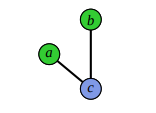
\includegraphics[scale=0.5]{Graphics/interferencegraph.png}
  \caption{An example of a coloured interference graph taken from \cite{ITU_liveness} }
  \label{fig:interferencegraph}
\end{figure}

In case there are too few registers/colours available to colour the interference graph, the excess values are \emph{spilled}, meaning that they are stored in memory instead.
